\documentclass[a4paper]{article}
\usepackage{graphicx, hyperref,amsmath,inputenc,gensymb}
\usepackage[dutch]{babel}
\usepackage[center]{caption}
\captionsetup[figure]{labelfont={bf,it},textfont=it}
\captionsetup[table]{labelfont={bf,it},textfont=it}

\begin{document}

\begin{titlepage}
  
  \begin{flushright}
	  
\includegraphics[width=6cm]{img/UHasseltorigineel.jpg}\\ 
    \Large 	Inleiding tot de sterrenkunde en astrofysica \\
    				Academiejaar 2014-2015\\
    				Prof. dr. Marc Gyssens
  \end{flushright}
    \vspace*{\fill}
    		\begin{center}
      		\Huge \bf De ringen van de reuzenplaneten\\[3cm]
    		\end{center}
    \vspace*{\fill}
  \begin{flushright}
    \Large
		Jeffrey Gorissen\\
		1436845\\
		1$^e$  bachelor fysica\\
		
  \end{flushright}
  
\end{titlepage}

\tableofcontents
\newpage

\section{Inleiding}
	De ringen van de giganten oftewel reuzenplaneten zorgen al sinds de opkomst van de astronomie 
    voor verwondering bij velen. Zo ook bij Galileo, die in 1610 een merkwaardige ontdekking deed en op 30 juli dit schreef:\\
    
\noindent
	``\textit{I discovered another very strange wonder, which I should like to make known to their Highnesses\ldots, 
		keeping it secret, however, until the time when my work is published\ldots the star of Saturn is not a single star, 
		but is a compsite of three, which almost touch each other, never change or move relative to each other, 
		and are arranged in a row along the zodiac, the middle one being three times larger than the lateral ones, 
		and they are situated in this form: oOo.}'' \\
		
\noindent
	Galileo zag dus niet onmiddelijk dat het ringen waren maar was toch beter op weg dan andere astronomen in zijn tijd.
	Die zagen Saturnus namelijk als een ovaal. Galileo verklaarde dat door het feit dat zij, in vergelijking met zijn materiaal,
	inferieure telescopen gebruikten. Het duurde echter tot 1659 voordat men het idee had
	dat het een ring kon zijn. Deze hypothese werd als eerste voorgesteld door Christiaan Huygens, een Nederlandse wetenschapper.
\section{Ringen}
Het is niet enkel de alom bekende Saturnus die ringen heeft. Ook Jupiter, Uranus en Neptunus hebben ringen. Dit komt echter doordat de ringen van Saturnus het meest uitgesproken zijn en
dan ook het best waarneembaar zijn zie Figuur \ref{fig:Saturnus} .
\begin{figure}[h]
	\centering 
	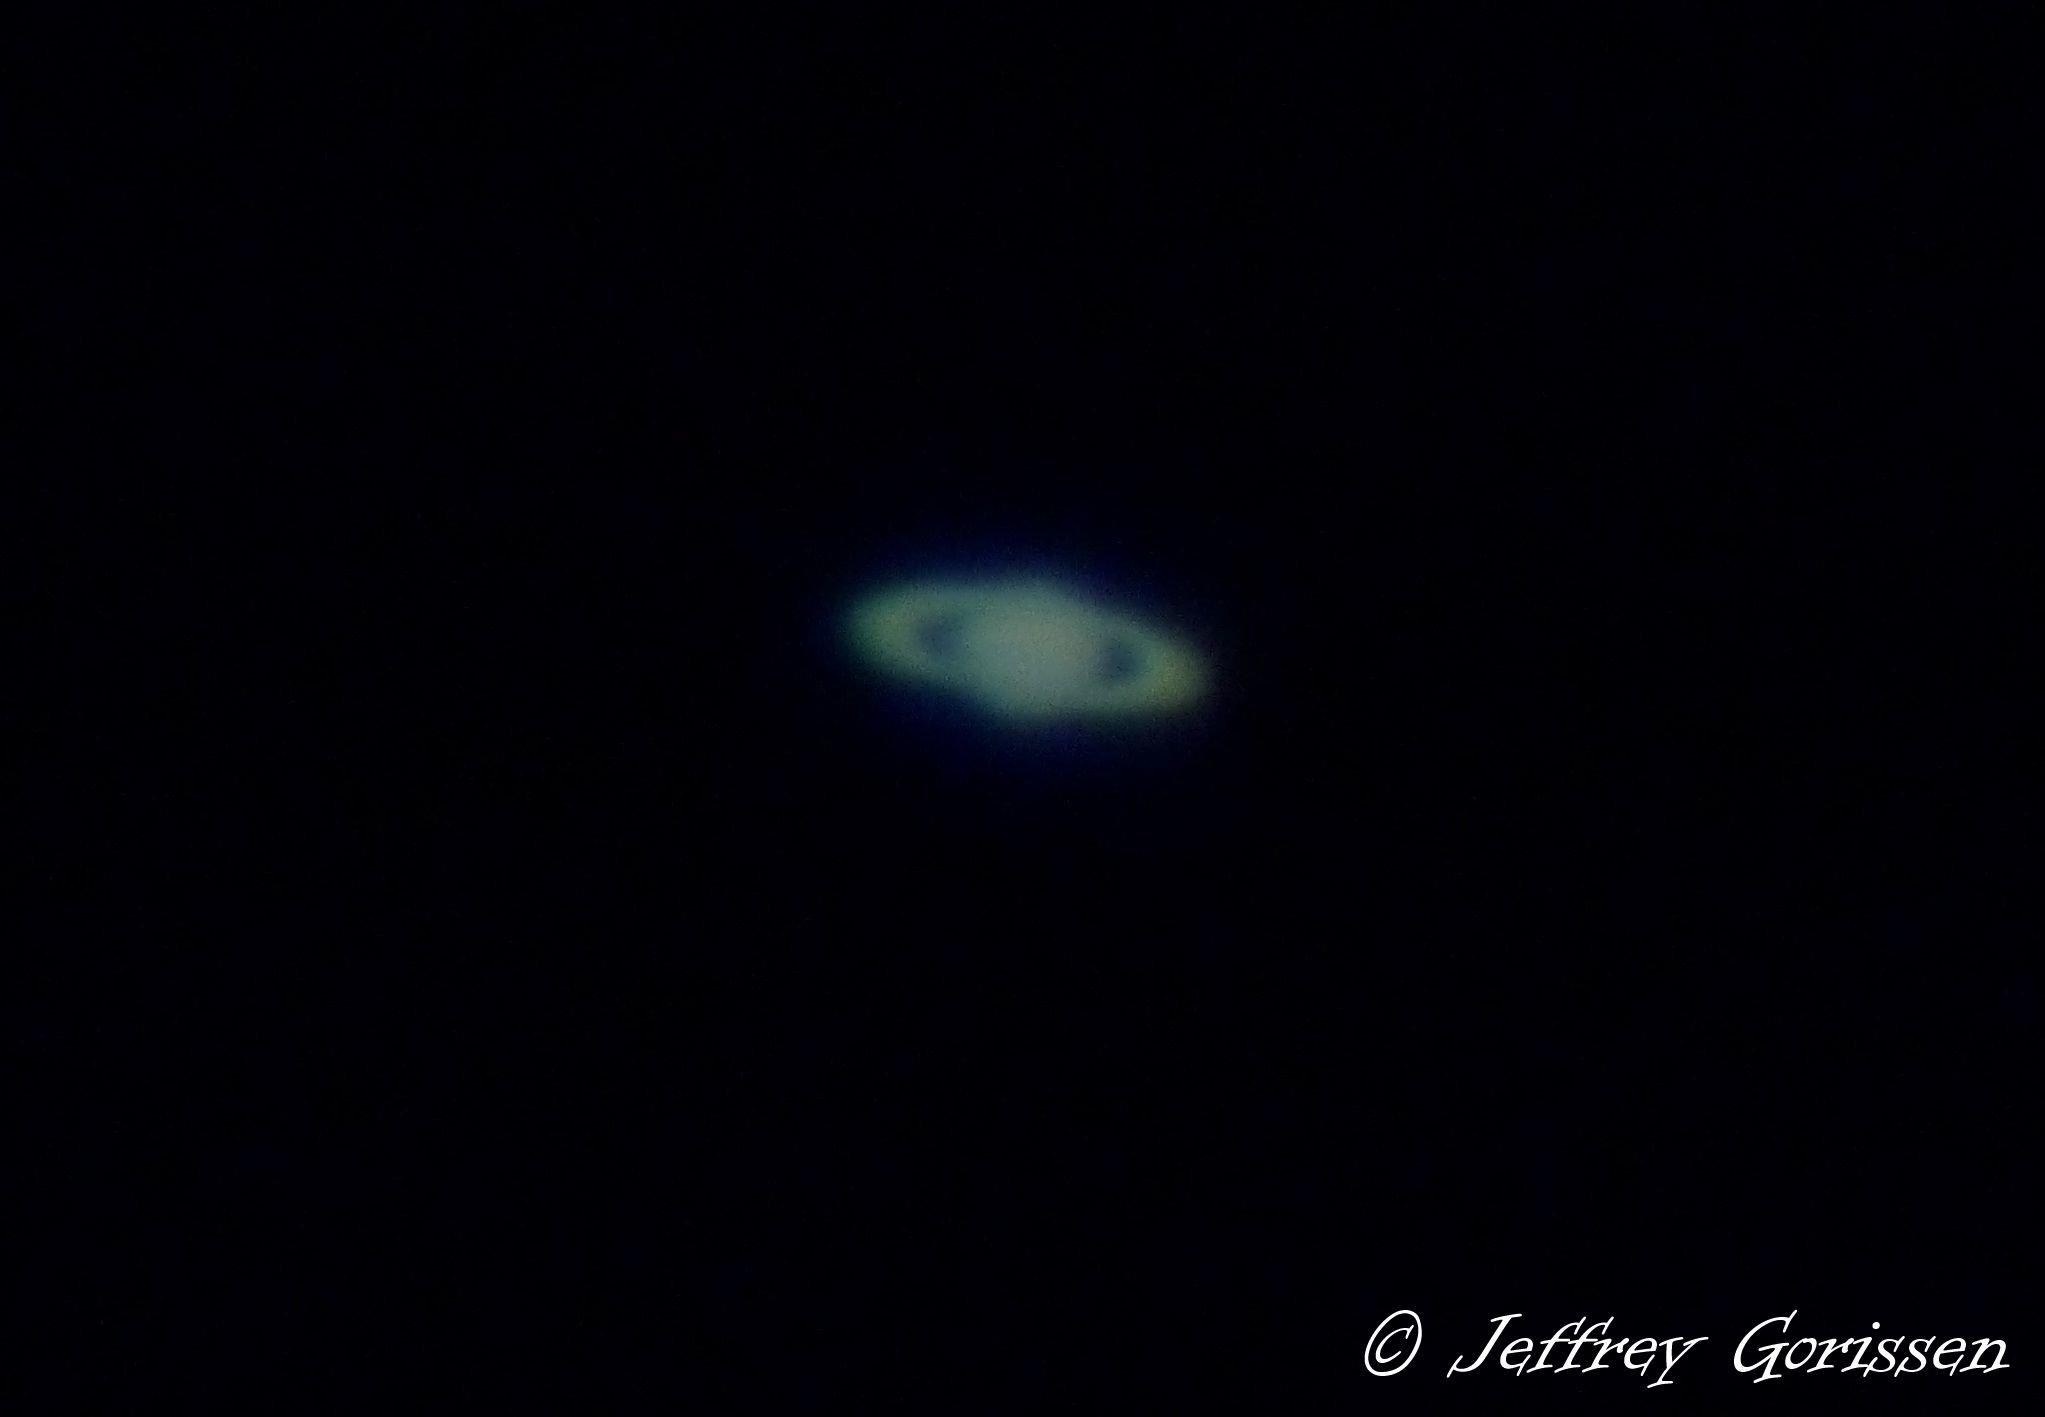
\includegraphics[scale=0.345]{img/goed-P1030276.JPG} 
	\caption{Een foto van Saturnus zoals te zien door een telescoop met een\newline lensopening van 90mm.}
	\label{fig:Saturnus}
\end{figure}
\newpage
	\subsection{Samenstelling}
	De ringen van Jupiter bestaan voornamelijk uit stof ([1]), waardoor ze ook veel moeilijker waar te nemen zijn dan die van Saturnus.
	Dit komt doordat ringen van Saturnus bestaan uit ijs en steen waarvan de omvang van de deeltjes sterk varieert in grootte: van zo klein als zandkorrels tot zo groot als complete huizen ([2]).
	Het ijs heeft namelijk een veel hogere reflectie van licht ten opzichte van stof en steen.
	De ringen van Neptunus zijn net zoals die van Jupiter veel donkerder dan die van Saturnus en dus ook moeilijker waar te nemen: ze zijn dus ook hoogstwaarschijnlijk opgebouwd uit steen en stof ([3]).
	Tot slot hebben de ringen van Uranus een gelijkaardige samenstelling als de ringen van Jupiter en Neptunus. Het ijs in de ringen van Saturnus, samen met de enorme grootte van de ringen zorgen ervoor dat
	de ringen van Saturnus het best waarneembaar zijn.\\
	\\
	Tabellen 1 tot en met 4 geven basale informatie over alle ringen per reuzenplaneet van ons zonnestelsel ([4][5]).
	Bij relatief kleine intervallen is soms enkel het maximum weergegeven om het overzicht te bewaren.
	 		 \begin{table}[h]
	 		 	\caption{ringen van Jupiter}
	 		 	\centering
	 		 	\begin{tabular}{l|lc|}
	 		 		\hline
	 		 		\multicolumn{1}{|l|}{\textbf{Naam}}          & \multicolumn{1}{l}{\textbf{Straal (km)}} & \multicolumn{1}{l|}{\textbf{Breedte (km)}} \\ \hline
	 		 		\multicolumn{1}{|l|}{Halo ring}              & 92 000 $-$ 122 500                           & 30 500                                      \\
	 		 		\multicolumn{1}{|l|}{Main ring}              & 122 500 $-$ 129 000                          & 6 500                                       \\
	 		 		\multicolumn{1}{|l|}{Amalthea gossamer ring} & 129 000 $-$ 182 000                          & 53 000                                      \\ 
	 		 		\multicolumn{1}{|l|}{Thebe gossamer ring}    & 129 000 $-$ 226 000                          & 97 000                                      \\ \hline
	 		 	\end{tabular}
	 		 \end{table}
	 	 \begin{table}[h]
	 	\caption{ringen van Saturnus}
	 	\centering
	 	\begin{tabular}{|l|cc|}
	 		\hline
\multicolumn{1}{|l|}{\textbf{Naam}}          & \multicolumn{1}{l}{\textbf{Straal (km)}} & \multicolumn{1}{l|}{\textbf{Breedte (km)}} \\ \hline
	 		D Ring                & 66 900 $-$ 74 510                  & 7 500          \\
	 		C Ring                & 74 658 $-$ 92 000                 & 17 500         \\
	 	    B Ring                & 92 000 $-$ 117 580                 & 25 500         \\
	 	    A Ring                & 122 170 $-$ 136 775               & 14 600         \\
	 		F Ring                & 140 180                             & 500          \\
	 		G Ring                & 166 000 $-$ 175 000                & 8 000          \\
	 		E Ring                & 180 000 $-$ 480 000                & 300 000          \\
	 		Phoebe Ring           & ~4 000 000 $-$ 13 000 000           & 
	 		\\ \hline
	 	\end{tabular}
	 \label{tab:2}
	 \end{table}
	 \begin{table}[h!]
	 	\caption{ringen van Uranus}
	 	\centering
	 	\begin{tabular}{|l|cc|}
	 		\hline
	 		\multicolumn{1}{|l|}{\textbf{Naam}}          & \multicolumn{1}{l}{\textbf{Straal (km)}} & \multicolumn{1}{l|}{\textbf{Breedte (km)}} \\ \hline
	 		$\zeta$cc   & 26 840 $-$ 34 890  & 8 000        \\
	 		$\zeta$c    & 34 890 $-$ 37 850  & 3 000        \\
	 		1986U2R     & 37 000 $-$ 39 500  & 2 500        \\
	 		$\zeta$     & 37 850 $-$ 41 350  & 3 500        \\
	 		6           & 41 837         & 2            \\
	 		5           & 42 234         & 5            \\
	 		4           & 42 570         & 4            \\
	 		$\alpha$    & 44 718         & 10           \\
	 		$\beta$     & 45 661         & 11           \\
	 		$\eta $     & 47 175         & 3            \\
	 		$\eta$c     & 47 176         & 40           \\
	 		$\gamma$    & 47 627         & 5            \\
	 		$\delta$c   & 48 300         & 12           \\
	 		$\delta $   & 48 300         & 6            \\
	 		$\lambda$   & 50 023         & 2            \\
	 		$\xi   $    & 51 149         & 100          \\
	 		$\nu$       & 66 100 $-$ 69 900  & 3 800        \\
	 		$\mu $      & 86 000 $-$ 103 000 & 17 000       \\ \hline
	 	\end{tabular}
	 \end{table}
	 \newpage
	 \begin{table}[h]
	 	\caption{ringen van Neptunus}
	 	\centering
	 	\begin{tabular}{|l|ll|}
	 		\hline
\multicolumn{1}{|l|}{\textbf{Naam}}          & \multicolumn{1}{l}{\textbf{Straal (km)}} & \multicolumn{1}{l|}{\textbf{Breedte (km)}} \\ \hline
	 		Galle (N42)      & 42 900   & 2 000            \\
	 		LeVerrier (N53)  & 53 200   & 113           \\
	 		Lassell          &  57 200  & 4 000            \\
	 		Arago            & 57 200   &  100 \\
	 		Adams (N63)      & 62 932   &  50         \\ \hline
	 	\end{tabular}
	 \end{table}
	 \subsection{Het tweelichamenprobleem}
	 	Het tweelichamenprobleem kent een analytische oplossing ([6]), in tegenstelling tot een drielichamenprobleem (of meer dan drie). Wat hiermee precies bedoeld wordt is dat het systeem van twee puntmassa's die interageren vanwege een zogenoemde centrale kracht exact beschreven kan worden ([7]), in het bijzonder de baan die de massa's volgen. Een centrale kracht is enkel afhankelijk van de afstand $r$ tussen de massa's, dus niet van de richting van beweging. Deze massa's zullen praktisch geen puntmassa zijn maar mits deze lichamen symmetrisch zijn, hebben zij de eigenschap alsof alle massa zich in \'{e}\'{e}n punt bevindt, namelijk in het centrum van het lichaam.\\
	 	
\noindent
Aangenomen dat er geen externe krachten zijn, zal het niets uitmaken welk assenstelsel of welke oorsprong gekozen wordt. De bewegingsvergelijkingen die het gehele systeem beschrijven volgen namelijk uit de zogenoemde Lagragiaan (het verschil tussen kinetische en potenti\"ele energie), welke invariant is onder een co\"ordinatentransformatie (theorema van Noether). Wanneer de kinetische energie dan beschreven wordt in termen van het massacentrum van het systeem en de oorsprong van het assenstelsel gekozen wordt in het massacentrum, speelt alleen het relatieve gedeelte van de Lagragiaan een rol. Dat wil zeggen: het niet-relatieve gedeelte, betreffende de kinetische energie van het massacentrum, kan worden weggelaten. Analoog aan een waarschijnlijk meer bekend mechanisch probleem: de kinetische energie is niet afhankelijk van de plaats, louter van de snelheid en de massa. Waar een bewegend lichaam gedefinieerd wordt is dan dus niet belangrijk.\\
	 	Nu geldt: 
	 	\begin{equation}
	 		\textbf{L} = \textbf{r} \times \textbf{p}
	 	\end{equation} 	(enkel vectori\"ele grootheden, $\times$ staat voor het kruisproduct ([8]))\\
	 	\textbf{L} is het draaimoment, \textbf{r} de relatieve positievector die het verschil tussen de posities van de betreffende lichamen voorstelt (dus \textbf{r} = $\mathbf{r_1} - \mathbf{r_2})$, en \textbf{p} de impuls van het relatieve systeem met  
	 	\begin{equation}
	 		\textbf{p} = \mu\textbf{v} = \frac{(m_1 m_2)}{(m_1+m_2)} \mathbf(\mathbf{v_1} - \mathbf{v_2})
	 	\end{equation}
	 	waarbij $m$ de massa en \textbf{v} naar de snelheid verwijst. \textbf{L}, \textbf{r} en \textbf{p} staan altijd loodrecht op elkaar gericht.
	 	Afleiden naar tijd toont hoe het draaimoment evolueert in de tijd:\\
	 	\begin{equation}
	 		\dfrac{d\mathbf{L}}{dt}  =  \dfrac{d}{dt} [\mathbf{r}\times\mathbf{p}]  =  \frac{d}{dt}t [\mathbf{r}\times\mu\mathbf{v}]  =  \frac{d\mathbf{r}}{dt}\times \mu \mathbf{v}+\mathbf{r}\times \mu \frac{d\mathbf{v}}{dt}
	 	\end{equation} 
	 	Maar $\dfrac{dr}{dt}$ = v, en $\mu\dfrac{dv}{dt}$ is massa maal versnelling, dit is de resulterende kracht $\mathbf{F}$ volgens de tweede wet van Newton, welke uiteraard gelijk is aan de centrale kracht. Deze centrale kracht staat in de richting van \textbf{r} zodat $\mathbf{F} = \mathbf{F}\times$ \textbf{\^r}, met \textbf{\^r} $= \dfrac{\mathbf{r}}{\mid \mathbf{r} \mid}$. Nu geldt voor kruisproducten: $\mid \mathbf{a} \times \mathbf{b}\mid = \mid \mathbf{a}\mid \mid \mathbf{b}\mid \sin\theta$, dus de grootte van het vectorieel product is gelijk aan het product van de grootte van de vectoren maal de sinus van de hoek tussen de vectoren.
	 	\begin{equation}
	 		\frac{d\mathbf{L}}{dt}   = \mathbf{v}\times \mu \mathbf{v}+\mathbf{r}\times F \textbf{\^r} ̂= \mu(\mathbf{v}\times\mathbf{v})+ \frac{F}{\mid \mathbf{r} \mid}(\mathbf{r}\times \mathbf{r})= \mu \mathbf{0}+\frac{F}{\mid \mathbf{r} \mid} \mathbf{0}=\mathbf{0}
		\end{equation}
	 	Want de hoek tussen twee dezelfde vectoren is 0 graden, zodat sin 0 = 0. De conclusie is dat het draaimoment niet verandert (evolueert) in de tijd. Het is een behouden grootheid.\\ \\
	 	Nu is reeds de oorsprong van het assenstelsel in het massamiddelpunt van het systeem gekozen. 
	 	Kies nu de richting van de (Cartesische) assen zodat $\mathbf{L}$=L\textbf{\^z}. 
	 	Aangezien \textbf{L} niet verandert zal \textbf{L} in de $z$-richting blijven wijzen. 
	 	Dus bewegen \textbf{r} en \textbf{p} zich in het $xy$-vlak. 
	 	Bijvoorbeeld: een planeet blijft in hetzelfde vlak roteren om een ster. 
	 	Dit is een gevaarlijk voorbeeld. De twee genoemde lichamen (planeet en ster) 
	 	bewegen ten opzichte van de oorsprong. Uiteraard, dit volgt uit de definitie van de 
	 	positievector \textbf{r} die een plaats (bijvoorbeeld in $xyz$-co\"{o}rdinaten) omschrijft waarbij gerefereerd wordt aan de oorsprong van het assenstelsel. Nu is het massamiddelpunt van het systeem gekozen als oorsprong. Een ster zal doorgaans zoveel meer massa hebben dan een planeet, zodat dit massamiddelpunt bijna samenvalt met de positie van de ster. Dus lijkt het alsof de ster niet beweegt en de planeet om de ster beweegt. Verder, twee lichamen hoeven niet te bewegen in een rotatie. Dit is slechts het gevolg van de initiële (kinetische) energie die de lichamen hebben. Zo zal het bijvoorbeeld afhankelijk zijn van de snelheid van een meteoro\"{i}de of de zwaartekracht van een ster deze meteoro\"{i}de zal kunnen binden in zijn omgeving. Gebonden beweging wordt beschreven door een ellips (dus rotatie) en ongebonden beweging door een hyperbool. Respectievelijk zijn de cirkel en de parabool extreme gevallen hiervan.
	\subsection{Baan van een planetaire ring}
	Een planetaire ring is een bijzonder lichaam. Per definitie bevindt dit lichaam zich overal in zijn eigen baan. Als de massa van de ring homogeen verdeeld is, dan is de overeenkomstige puntmassa gelokaliseerd in het middelpunt van de planeet. Het massamiddelpunt van het systeem bevindt zich dus ook in het middelpunt van de planeet, en bijgevolg beweegt de ring zich om de planeet. Deze beweging zal een rotatie blijven vanwege het behoud van draaimoment, op voorwaarde dat er geen externe krachten deze beweging verstoren.\\
	
\noindent
Zo'n externe kracht is de centrifugaalkracht. Dat klinkt niet als een externe kracht, maar het is geen centrale kracht behorend bij het tweelichamenprobleem. Vanwege de rotatie van de planeet zal de massa van de planeet vlieden naar de buitenkant ([9]). Deze middelpuntvliedende kracht is het sterkst aan de evenaar, waar de rotatiesnelheid (in meter per seconde, niet radialen per seconde) het grootst is. Gevolg is dat de planeet rond de evenaar breder wordt en de polen afgeplat worden. Deze vormverandering is afhankelijk van het verschil tussen zwaartekracht (die de massa sferisch vormt) en middelpuntvliedende kracht (die de massa in een schrijf wil doen vormen). Zowel een sfeer als een schijf hebben hetzelfde massamiddelpunt dus de puntmassa van de planeet behoudt dezelfde positievector. Echter zal deze vormverandering ervoor zorgen dat het baanvlak van de ring gelijk is aan het evenaarsvlak van de planeet. Want aan de evenaar is de massa het grootst zodat deze een grotere zwaartekracht uitoefent op de ring dan elders.\\

\noindent
Bij Saturnus en Uranus is dit duidelijk te zien. Saturnus heeft een obliquiteit van ongeveer 27\degree. Met andere woorden: de rotatie-as van Saturnus maakt een hoek van 27\degree met het baanvlak van deze planeet ([10]). Het baanvlak van de ringen van Saturnus maakt deze zelfde hoek met het baanvlak van de planeet. Dus de ringen bewegen om de evenaar. Nog duidelijker is dit bij Uranus, die een obliquiteit heeft van ongeveer 98\degree, zie Figuur \ref{fig:uranus} :
	\begin{figure}[h]
		\centering
		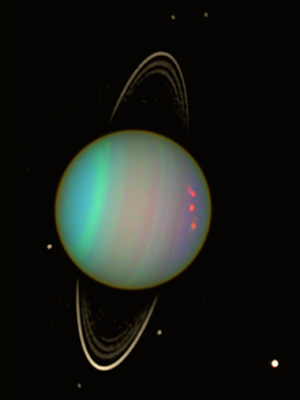
\includegraphics[scale=0.43]{img/uranus.jpg}
		\caption{Uranus en haar ringen gefotografeerd vanuit het baanvlak van de planeet ([11]). Alle ringen draaien om Uranus in een vlak dat minder dan 0,1\degree verschilt met het evenaarsvlak van de planeet.}
		\label{fig:uranus}
	\end{figure}
	De aanwezigheid van andere lichamen zorgen ook voor een externe kracht. Zij oefenen ook een zwaartekracht $F_z$ uit vanwege hun massa ([12]):
	\begin{equation}
	F_z=G\frac{m_1 m_2}{r^2}
	\end{equation}
	Met $G$ de gravitatieconstante, $m_1$ en $m_2$ de massa’s van lichamen, en r de afstand tussen de massacentra van de lichamen. Punt is dat $F_z \propto r^{-2}$, wat er op neer komt dat alleen lichamen die in de buurt zijn er echt toe doen, en alleen lichamen met een massa die,relatief aan de planeet in kwestie, niet zeer klein is. Planetaire manen kunnen zich hier voor kwalificeren. De ring kan hierdoor vervormen, maar de ringvorm kan ook juist behouden blijven. In dit laatste geval wordt van zogenoemde ``shepherd moons'' gesproken ([13]). De zwaartekracht van zo'n maan kan materiaal dat uit de ring kwam afbuigen zodat het materiaal weer terug in de ring kan komen. Of het materiaal komt op de maan terecht zodat de afwijkende baan van het betreffende ringmateriaal niet meer bestaat, of het materiaal wordt afgebogen in een hyperbolische baan zodat het ongebonden wordt en het systeem verlaat. De Adams-ringen van Neptunus zijn bijvoorbeeld zeer stabiel vanwege de aanwezigheid van de shepherd moon Galatea ([14]).\\
	
\noindent
	Weer een andere externe kracht is een botsing. Zo is een meteoro\"ide waarschijnlijk ingeslagen op de hoofdring van Jupiter, waardoor deze ring zich niet alleen in een vlak beweegt, maar ook een (verticale) golfbeweging heeft ([15]).\\
	
\noindent
	De Phoebe-ring van Saturnus heeft een afwijkende baan ([16]), zoals in Tabel \ref{tab:2} te zien is. De afstand tussen het centrum van Saturnus en de Phoebe-ring varieert van 4 tot 13 miljoen kilometer, net binnen de baan van Phoebe ([17]). Een aanblik van Phoebe doet vermoeden dat er veel inslagen geweest zijn, zie Figuur~\ref{fig:Phoebe}. De Phoebe-ring was dan ook waarschijnlijk geformeerd uit materiaal van Phoebe. Terwijl Saturnus zoals gezegd een obliquiteit van 27\degree heeft, is dit 5\degree voor Phoebe en de Phoebe-ring. Hierdoor ziet men de helft van de ring boven het evenaarsvlak van Saturnus en de andere helft eronder. Zonder externe krachten kan de Phoebe-ring weliswaar in het evenaarsvlak van Saturnus komen, maar dit kan miljoenen jaren duren.
	\begin{figure}[h]
		\centering 
		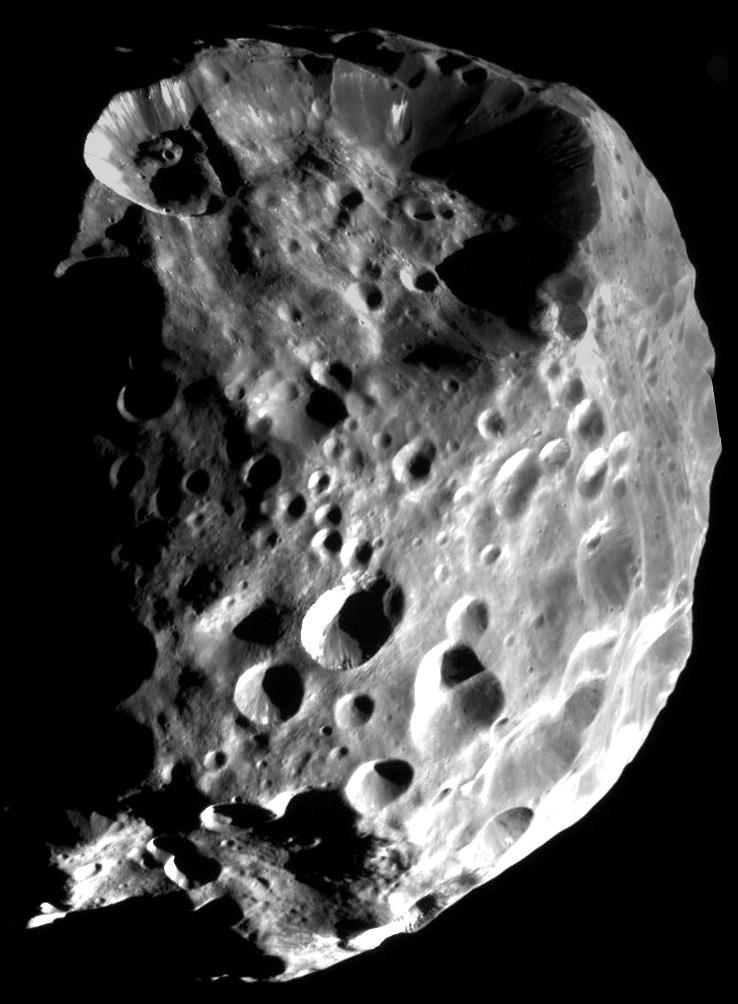
\includegraphics[scale=0.21]{img/Phoebe.jpg}
		\caption{De maan van Saturnus, Phoebe.}
		\label{fig:Phoebe} 
	\end{figure}
	\newpage
	\subsection{Ontdekking en ontstaan van de ringen}
		\subsubsection{Jupiter}
		De ringen van Jupiter werden in 1970 ontdekt door de eerste sondes die Jupiter bezochten.
		De ringen lijken te zijn ontstaan door inslagen op kleine maantjes waardoor stof en gruis terecht gekomen zouden zijn in een baan rond Jupiter ([1]). Jupiter zelf is te zien op Figuur \ref{fig:JupiterRedDot}.
		\subsubsection{Saturnus}
		De ringen van Saturnus zijn voor het eerst waargenomen door Galileo Galilei in 1610 zoals eerder al vermeld. Later zijn deze ringen
		in de jaren 80 nog in detail bestudeerd door Voyager 1 en 2. De ringen zijn alfabetisch benoemt in de volgorde van ontdekking, zie ook Figuur \ref{fig:SaturnusGelabeled}. Dit is in het
		begin misschien vreemd want hierdoor is de binnenste ring de D ring, en niet A ook al lijkt dat logischer. De informatie van NASA's Cassini missie
		zal ons laten zien hoe de ringen zich gevormd hebben, hoe ze hun baan rond Saturnus behouden en waarom ze er in de eerste plaats zijn ([18]). Mogelijk zijn de ringen volledig ontstaan door manen die `verslonden' werden,
		zie ook Figuur \ref{fig:Krantensnipsel} in de Appendix.
		\subsubsection{Uranus}
		De ringen van Uranus zijn in het jaar 1977 ontdekt door James L. Elliot, Edward W. Dunham, en Jessica Mink. Ze waren aan het observeren hoe Uranus
		voor een ster schoof toen ze opmerkten dat de ster leek te knipperen, dit werd natuurlijk veroorzaakt door 
		de ringen die het licht blokkeerde. Later in 1986 kon ook Voyager 2 de ringen van Uranus bevestigen ([19]).
		Over het ontstaan is er echter nog niets gekend.
		\subsubsection{Neptunus}
		Na bewijzen voor het bestaan van de ringen van Neptunus midden jaren 80, zijn er in 1989
		foto's genomen door Voyager 2 die wederom een bevestiging gaven over het bestaan van ringen bij de reuzenplaneten ([20]).
		Over het ontstaan zijn echter ook bij Neptunus nog geen theorie\"en.

	
\section{Rochelimiet}
Zoals eerder vermeld bestaan ringen in het algemeen uit kleine deeltjes zoals stof en ijs. Het is dan ook plausibel om aan te nemen dat deze deeltjes afkomstig zijn van satellieten die afgebroken zijn wegens de aantrekkingskracht van de planeet. Men kan zich dan ook onmiddellijk  afvragen wanneer (lees: de afstandslimiet tot de planeet) dergelijke satellieten afbreken. In 1848 werd deze vraag beantwoord door \'{E}douard Roche aan de hand van een theoretisch bepaalde limiet, de Rochelimiet. In deze tekst worden enkele vereenvoudigde gevallen besproken en aangetoond.

\subsection{Starre lichamen in een cirkelvormige baan}
Veronderstel een sferische, starre satelliet met massa $m$ die zich in een cirkelvormige baan rond een planeet met massa $M$ en straal $R$ bevindt. Veronderstel ook dat deze satelliet een hydrostatisch equilibrium aanneemt. Men kan nu de Rochelimiet voor deze planeet bepalen aan de hand van een mathematische truc, namelijk door de wetten van Newton toe te passen op een fictieve massa $m'$ op de oppervlakte (de kant die het dichtst bij de planeet staat) van de satelliet.\\

\noindent
Uit de gravitatiewet van Newton weet men dat de aantrekkingskracht tussen de fictieve massa en de satelliet als volgt wordt uitgedrukt:
	\begin{equation}
	F_z = G\frac{mm'}{r^2}
	\end{equation}
met $G$ de gravitationele constante en $r$ de afstand tussen de massacentra van de fictieve massa en de satelliet.\\

\noindent
Anderzijds bevindt de fictieve massa zich ook nog in een getijdenveld, dus werkt er een getijdenkracht van de planeet op de fictieve massa. Deze kracht kan men vinden door het verschil te nemen tussen aantrekkingskracht van de planeet op het centrum van de satelliet en de aantrekkingskracht van de planeet op de dichtstbijzijnde rand van de satelliet. In wiskunde symbolen geeft dit
	\begin{align}
	F_g &= G\frac{Mm'}{(d-r)^2} - G\frac{Mm'}{d^2}\\
	&= GMm'\frac{2dr-r^2}{d^4 - 2d^3r +r^2 d^2}
	\end{align}	 
met $d$ de afstand tussen de massacentra van de planeet en de satelliet. Gebruik makende van het feit dat $R>>r$ en $d>>R$, verkrijgt men de volgende benadering:
	\begin{equation}
	F_g = G\frac{2Mm'r}{d^3}
	\end{equation}\\
	
\noindent
Omdat de satelliet een cirkelvormige baan rond de planeet beschrijft, speelt er in de krachtenwerking ook nog een centrifugale kracht mee. De centrifugale kracht, gebruik makende van de derde wet van Kepler en $M>>m$, op de fictieve massa wordt gegeven door
	\begin{equation}
	F_c = G\frac{Mm'r}{d^3}
	\end{equation}
Merk op dat deze kracht wordt opgeteld bij de getijdenkracht. Volgens de wetten van Newton heeft men dan
\begin{align}
F_z &= F_g + F_c\\
G\frac{mm'}{r^2} &= G\frac{3Mm'r}{d^3}
\end{align}
Bijgevolg kan men de volgende uitdrukking voor $d$ vinden:
\begin{equation}
d = r\sqrt[3]{3\frac{M}{m}}
\end{equation}
Omdat het werken met deze formule onhandig is wegens het feit dat $r$ aanwezig is in de uitdrukking, herschrijft men de massa's aan de hand van hun symmetrie:
\begin{equation}
M = \frac{4\pi \rho R^3}{3}
\end{equation}
\begin{equation}
m = \frac{4\pi\rho' r^3}{3}
\end{equation}
met $\rho$ de massadichtheid van de planeet en $\rho'$ de massadichtheid van de satelliet. Men verkrijgt nu een mooie uitdrukking voor de Rochelimiet ([21]):
\begin{equation}
d = R\sqrt[3]{3\frac{\rho}{\rho'}}
\end{equation}
Men kan nu onmiddellijk zien dat $d \propto \sqrt[3]{\dfrac{\rho}{\rho'}}$.

\subsection{Vloeibare satellieten}
Aan de andere kant van het spectrum bevinden zich vloeibare satellieten met een synchrone rotatie. Deze satelliet wordt veel sneller vervormd door het getijdenveld waardoor het een sfero\"{i}de wordt. De afleiding voor de limiet is meetkundig zeer complex waardoor het bewijs hier weggelaten wordt. Roche heeft een niet- exacte berekening gegeven:
\begin{equation}
d \approx 2,44\sqrt[3]{\frac{\rho}{\rho'}}
\end{equation}
Men kan echter met de computer betere benaderingen vinden die rekening houden met de vorm van de satelliet.



\newpage
\section{Appendix}
	\begin{figure}[h]
		\centering
		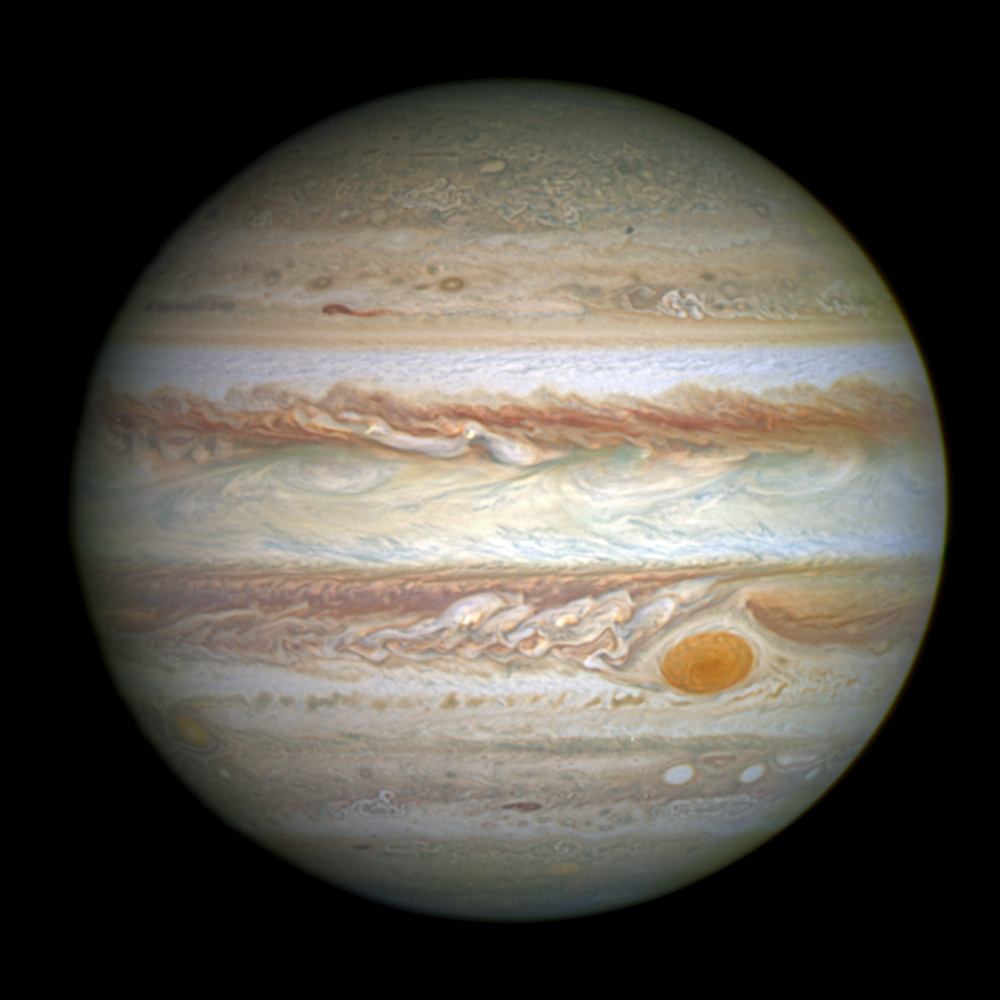
\includegraphics[scale=0.24]{img/JupiterRedDot.jpg}
		\caption{Foto van Jupiter gemaakt door de Hubble Space Telescope.}
		\label{fig:JupiterRedDot}
	\end{figure}

	\begin{figure}[!h]
			\centering
			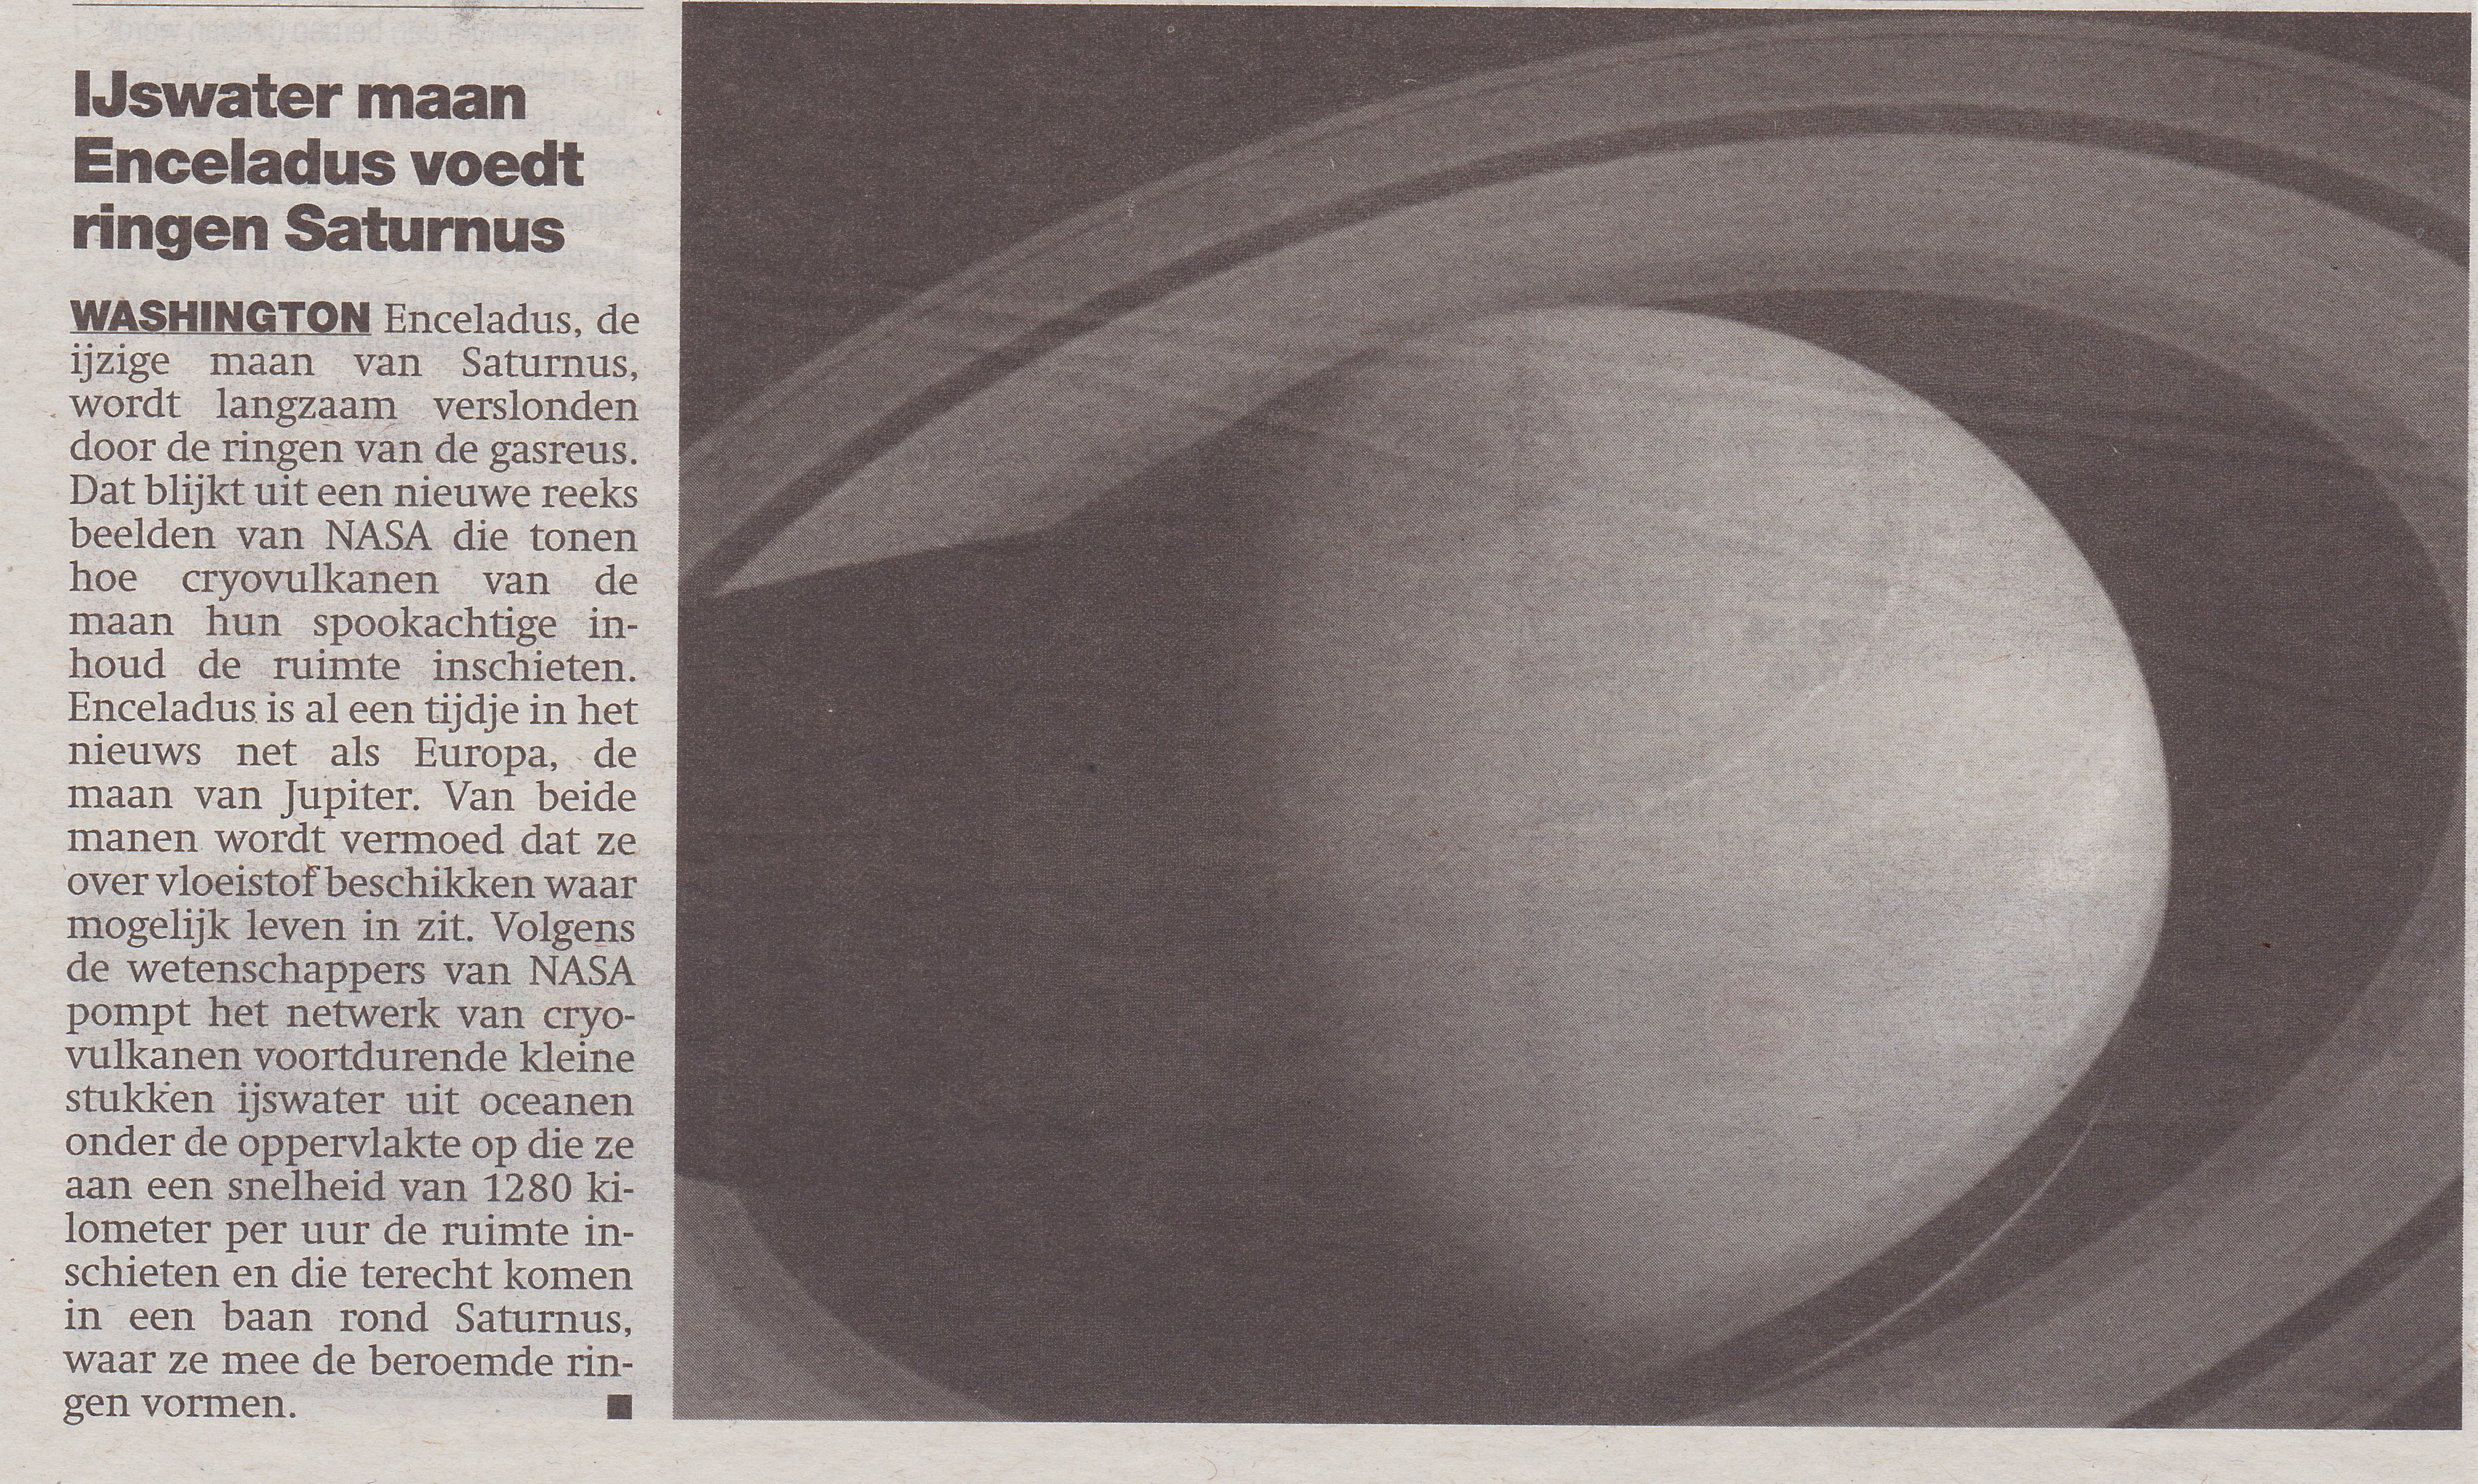
\includegraphics[scale=0.72]{img/Krantensnipsel.jpg}
			\caption{Krantenartikel uit ``Metro'' van dinsdag 21 april 2015 (Nr. 3179): Hoe de ringen waarschijnlijk zijn ontstaan en hoe ze in stand gehouden worden.}
			\label{fig:Krantensnipsel}
	\end{figure}
	\begin{figure}[!p]
			\centering
			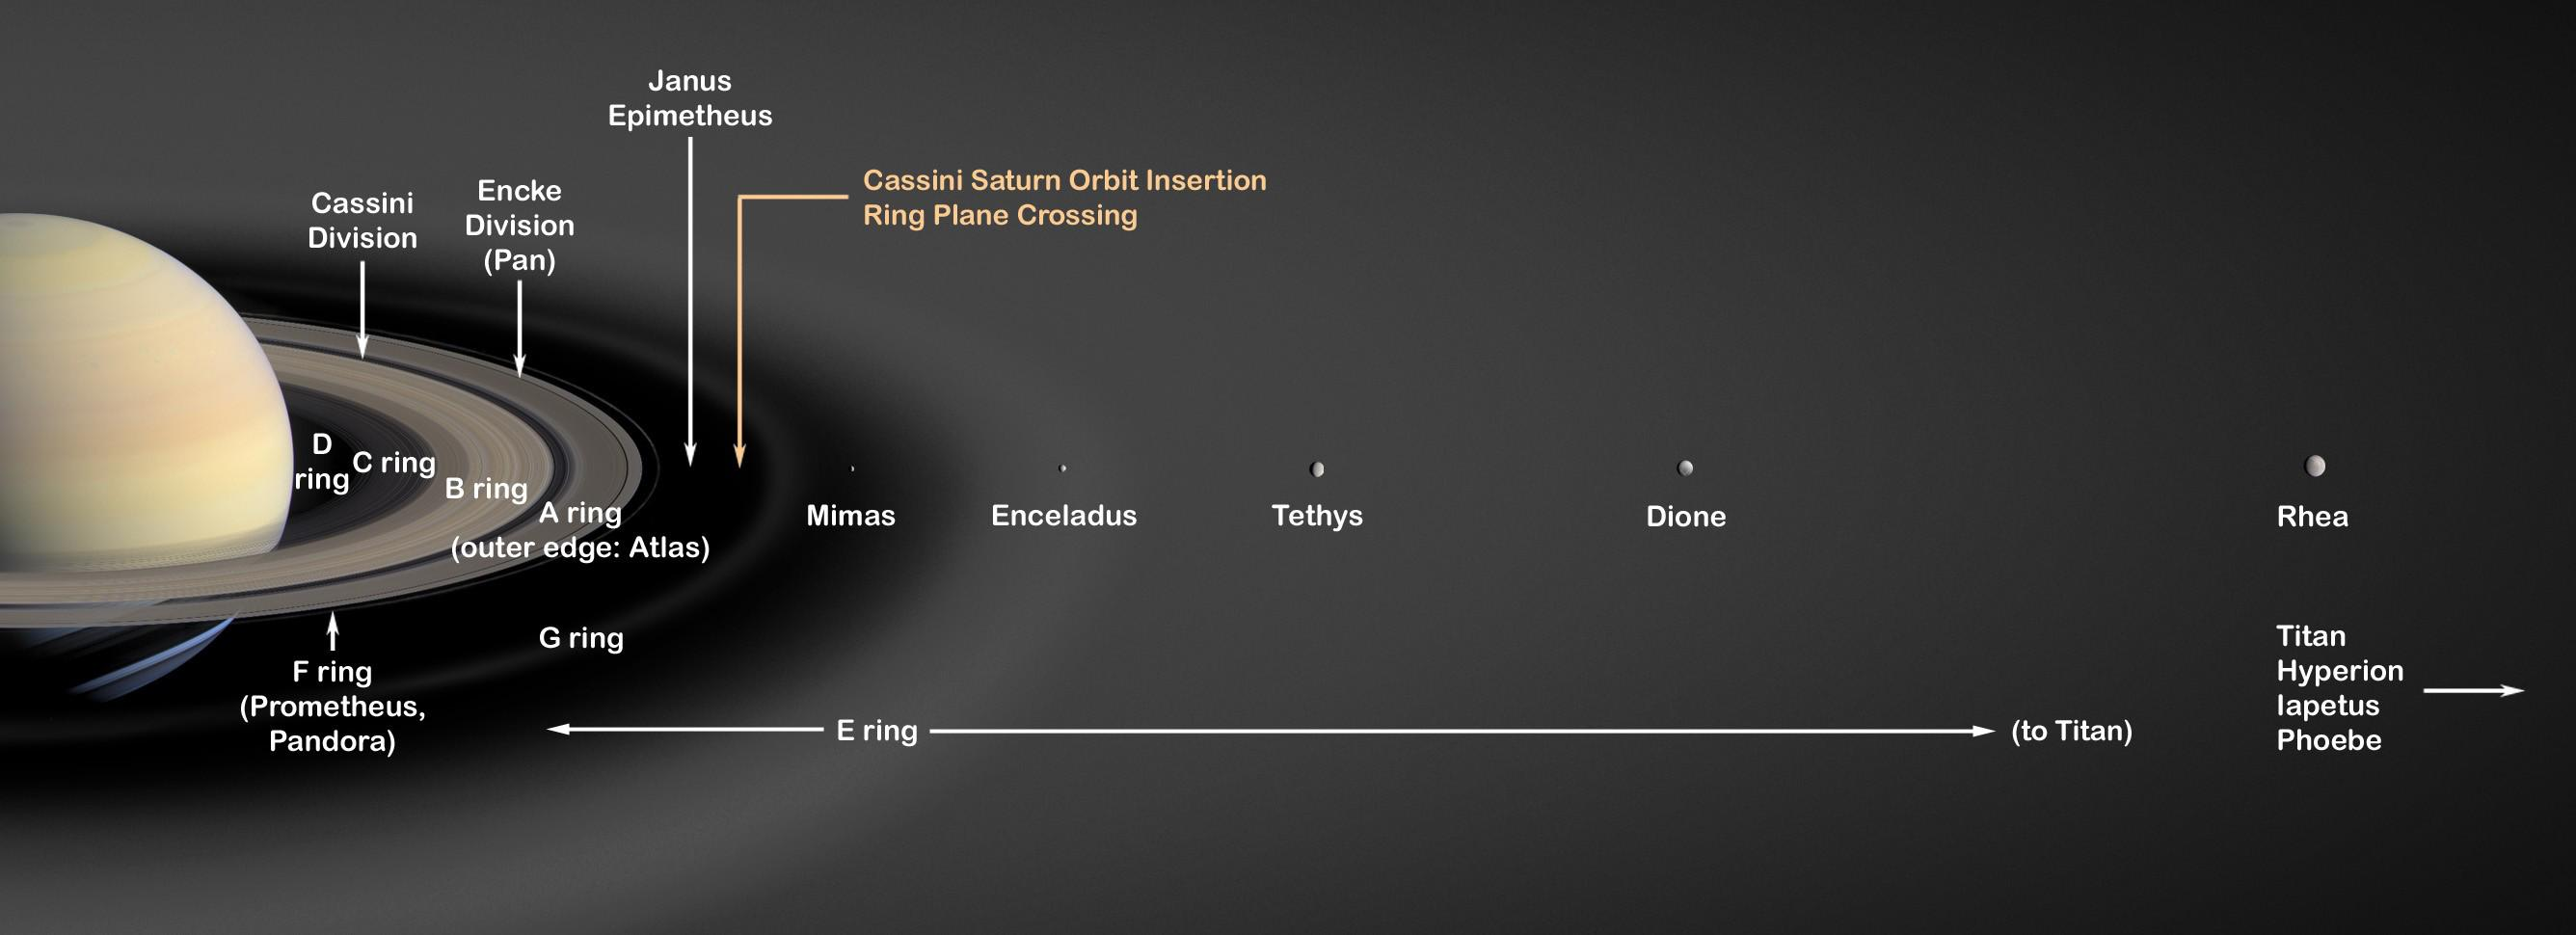
\includegraphics[scale=0.21, angle=90]{img/SaturnusGelabeled.jpg}
			\caption{Zijaanzicht van het Saturnussysteem met namen van ringen en manen (afbeelding zonder copyright).}
			\label{fig:SaturnusGelabeled}
	\end{figure}
	
	\newpage
\section{Bronnen}	
Internetbronnen zijn geraadpleegd in april en mei 2015.\\

\noindent\text{[1]} \url{https://solarsystem.nasa.gov/planets/profile.cfm?Object=Jupiter&Display=Rings}\\
\text{[2]} \url{https://www.nasa.gov/audience/forstudents/k-4/stories/ring-a-round-the-saturn.html#.VVc1D5ftlBc}\\
\text{[3]} \url{http://www.windows2universe.org/neptune/moons_and_rings.html}\\
\text{[4]} Gazetteer of Planetary Nomenclature, \url{http://planetarynames.wr.usgs.gov/Page/Rings}\\
\text{[5]} NASA, \url{http://nssdc.gsfc.nasa.gov/planetary/factsheet/} \\
\text{[6]} Gyssens, Inleiding tot de sterrenkunde en astrofysica, Universiteit Hasselt, 2014/2015 \\
\text{[7]} Hand and Finch, Analytical Mechanics, Cambridge University Press, New York, 7th printing (2008) WW
\text{[8]} Adams and Essex, Calculus a complete course, Pearson Canada Inc., Toronto, 7th ed. (2010) \\
\text{[9]} \url{http://saturn.jpl.nasa.gov/faq/FAQSaturn/#q14} \\
\text{[10]} NASA, \url{http://nssdc.gsfc.nasa.gov/planetary/planetfact.html} \\
\text{[11]} E.C. Stone, E.D. Miner. Voyager 2 encounter with the uranian system. Science 233 (1986) 39–43 \\
\text{[12]} Young and Freedman, Sears and Zemansky’s University Physics with modern physics, Pearson Education inc., San Fransisco, 13th ed. (2012) \\
\text{[13]} The Planetary Society, \url{http://www.planetary.org/blogs/emily-lakdawalla/2014/07010001-ringmoons-shepherds.html} \\
\text{[14]} University of Maryland, \url{http://www.astro.umd.edu/~hamilton/research/preprints/BurHamSho01.pdf} \\
\text{[15]} Ciclops, \url{http://www.ciclops.org/view.php?id=6762&js=1} \\
\text{[16]} The Planetary Society, \url{http://www.planetary.org/blogs/emily-lakdawalla/2009/2165.html} \\
\text{[17]} NASA, \url{www.jpl.nasa.gov/news/news.cfm?release=2009-150}\\
\text{[18]} \url{https://solarsystem.nasa.gov/planets/profile.cfm?Object=Saturn&Display=Rings}\\
\text{[19]} \url{https://solarsystem.nasa.gov/planets/profile.cfm?Object=Uranus&Display=Rings}\\
\text{[20]} \url{https://solarsystem.nasa.gov/planets/profile.cfm?Object=Neptune&Display=Rings}\\
\text{[21]} \url{http://www.jgiesen.de/astro/stars/roche.htm}
\end{document}